\smartsection{Advanced Features}
\label{sec:advanced-features}

\smartsubsection{Overview}

This section covers the assignment's Part~4 requirements (25 points):
Guard Mode, black-box logging, a software watchdog, and adaptive thermal
management. All four are implemented inside the existing
\texttt{surveillance\_notifier} daemon from Section~\ref{sec:mqtt-email}
rather than as four new processes.

\begin{table}[H]
\centering
\caption{Where each feature lives.}
\label{tab:advanced-locations}
\resizebox{\textwidth}{!}{%
\begin{tabular}{lll}
\toprule
\textbf{Feature} & \textbf{Enforcement / decision} & \textbf{Toggle / applied by} \\
\midrule
Guard Mode & \texttt{surveillance\_notifier} (\texttt{main.c}) & Toggle: Section~\ref{sec:rest-api}'s \texttt{api\_router.c} / dashboard \\
Black box (SQLite) & \texttt{surveillance\_notifier} (\texttt{black\_box.c}) & Read: Section~\ref{sec:rest-api}'s REST API \\
Watchdog & \texttt{surveillance\_notifier} (\texttt{watchdog.c} + \texttt{service\_ctl.c}) & --- \\
Adaptive thermal & \texttt{surveillance\_notifier} (\texttt{thermal.c}) & Applied mechanically by \texttt{person\_detector.py} \\
\bottomrule
\end{tabular}
}
\end{table}

\begin{questionsection}{Why route all four features through one existing daemon instead of building them as separate processes?}
Guard Mode, the watchdog, and thermal management all need to send e-mail
alerts, and Section~\ref{sec:mqtt-email} already established a single
30-second debounce clock for exactly that purpose.
\end{questionsection}

\begin{answersection}{One shared debounce, one honest guarantee}
Four independently-debounced processes would not add up to one
rate-limited system --- each would honestly enforce "at most one email
per 30 seconds" \emph{from itself}, while the system as a whole could
still send up to four emails in the same 30-second window. Routing plain
detection, Guard Mode alarms, watchdog timeouts, and thermal throttle
events through the exact same \texttt{should\_send\_email()}
(Listing~\ref{code:debounce}) keeps the debounce guarantee meaningful at
the system level, not just per-trigger. Black-box logging makes the
\emph{opposite} choice on purpose: it is never debounced, since its job
is to be a complete record even during a debounce-suppressed burst ---
every detection, alarm, timeout, and throttle event is logged regardless
of whether an e-mail actually went out for it.
\end{answersection}

\smartsubsubsection{Cross-process state}

Following the same IPC pattern used throughout the project
(\texttt{frame.jpg}/\texttt{persons.json} in
Section~\ref{sec:image-processing}), three more small files/databases
under \texttt{/dev/shm/surveillance/} tie the pieces together:

\begin{itemize}
    \item \texttt{guard\_state.json} --- written by
    Section~\ref{sec:rest-api}'s REST API
    (\texttt{POST /api/v1/guard \{"enabled": true\}}, which is exactly
    what the dashboard's toggle button calls via JS \texttt{fetch} ---
    "toggle via API or page" is one implementation, not two); read-only
    to this daemon.
    \item \texttt{control.json} --- written by this daemon's
    \texttt{thermal.c} whenever the throttle state changes;
    \texttt{person\_detector.py} polls it every $\sim$2\,s and
    mechanically applies whatever \texttt{target\_fps}/
    \texttt{processing\_scale} it contains, with no thermal logic of its
    own.
    \item \texttt{blackbox.db} --- SQLite in WAL mode, written by this
    daemon directly via the SQLite C API (never the \texttt{sqlite3}
    CLI); opened read-only by Section~\ref{sec:rest-api}'s REST API for
    \texttt{GET /api/v1/blackbox/*}.
\end{itemize}

\smartsubsection{Guard Mode}

While armed, a new detection (\texttt{count} $\geq 1$) does two things
\emph{immediately}, plus one debounced thing:

\begin{itemize}
    \item Publishes to \texttt{home/<student\_id>/alarm} at QoS~1 ---
    \punder{not} debounced, since the whole point of an alarm topic is
    immediacy; only the e-mail channel is rate-limited by spec.
    \item Logs a \texttt{guard\_alarm} event to the black box ---
    likewise never debounced (see above).
    \item Sends a \texttt{GUARD MODE ALARM} e-mail through the shared
    30-second debounce.
\end{itemize}

\begin{figure}[H]
\centering
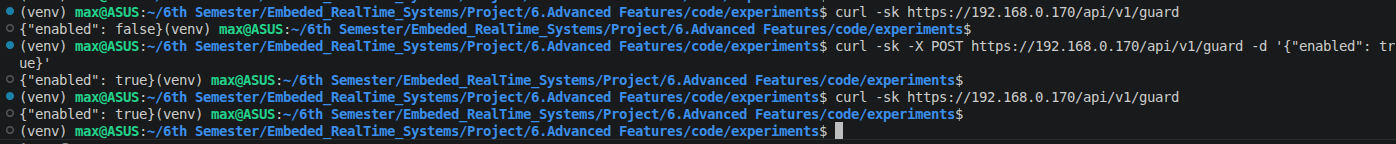
\includegraphics[width=0.9\textwidth]{../../6.Advanced Features/results/fig/GuardMode-Toggle-API.png}
\caption{Toggling Guard Mode via the REST API: initial state \texttt{false}, armed with a \texttt{POST}, confirmed \texttt{true} on the next \texttt{GET}.}\label{fig:guard-toggle-api}
\end{figure}

\begin{figure}[H]
\centering
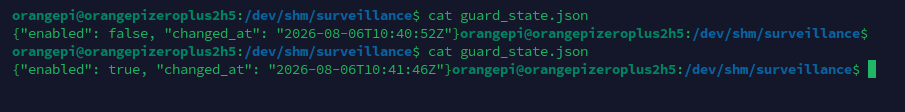
\includegraphics[width=0.8\textwidth]{../../6.Advanced Features/results/fig/GuardMode-Toggle-Result.png}
\caption{\texttt{guard\_state.json} on disk before and after the toggle above, including the \texttt{changed\_at} timestamp the daemon reads.}\label{fig:guard-toggle-result}
\end{figure}

\smartsubsection{Black Box (SQLite)}

\begin{lstlisting}[style=cstyle_bright_2026, caption={\texttt{black\_box.c} --- schema. WAL mode is used specifically because this process writes every poll cycle while a report screenshot might query the same file concurrently.}, label={code:blackbox-schema}]
"CREATE TABLE IF NOT EXISTS events ("
"  id INTEGER PRIMARY KEY AUTOINCREMENT,"
"  event_type TEXT NOT NULL,"
"  timestamp TEXT NOT NULL,"
"  person_count INTEGER,"
"  cpu_temp_c REAL,"
"  detail TEXT"
");"
"CREATE TABLE IF NOT EXISTS meta ("
"  key TEXT PRIMARY KEY,"
"  value INTEGER NOT NULL"
");"
"INSERT OR IGNORE INTO meta (key, value) VALUES ('total_events_ever', 0);"
\end{lstlisting}

Two tables, deliberately doing two different jobs: \texttt{events} is a
circular buffer capped at \texttt{blackbox\_max\_events} (default 1000)
--- every insert past the cap deletes the oldest row(s) first --- while
\texttt{meta.total\_events\_ever} is a counter that is \keyterm{never
trimmed}. This directly answers the assignment's "queryable
total-detection-count" requirement unambiguously: the \texttt{events}
table alone cannot answer "how many, ever" once it has wrapped around and
begun overwriting old rows.

\begin{figure}[H]
\centering
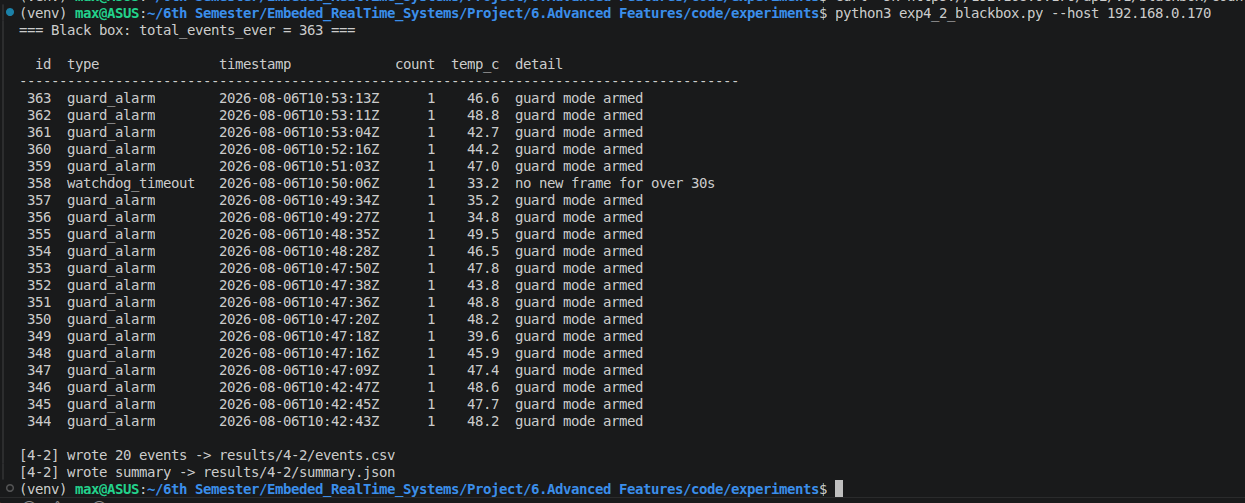
\includegraphics[width=0.95\textwidth]{../../6.Advanced Features/results/fig/GuardMode-Blockbox.png}
\caption{\texttt{exp4\_2\_blackbox.py} pretty-printing the black box during a Guard Mode session: 363 total events ever recorded, most-recent rows showing a mix of \texttt{guard\_alarm} and one \texttt{watchdog\_timeout} entry.}\label{fig:blackbox-query}
\end{figure}

\smartsubsection{Watchdog}

\texttt{person\_detector.py}'s own capture loop never exits on a failed
read (it logs and continues indefinitely), so
\texttt{Restart=on-failure} on \texttt{surveillance-imgproc.service}
would never fire on its own even with a genuinely dead feed --- this
daemon has to notice the staleness from the \emph{outside}.

\begin{lstlisting}[style=cstyle_bright_2026, caption={\texttt{watchdog\_check()} --- fires once per stale period, not on every poll cycle while already stale.}, label={code:watchdog-check}]
int stale_seconds = (int)(now - state->last_change_epoch);
if (stale_seconds > timeout_seconds && !state->timeout_fired) {
    state->timeout_fired = 1; /* fire once per stale period */
    /* ... log watchdog_timeout, send alert email,
           service_ctl_restart("surveillance-imgproc") ... */
}
\end{lstlisting}

The restart itself goes through \texttt{service\_ctl.c}, which calls
\texttt{execvp("systemctl", ...)} against a fixed \texttt{argv} array ---
never a shell string built from concatenated text --- the same safe
pattern already used for Section~\ref{sec:rest-api}'s bonus
\texttt{/api/v1/services/*} endpoints.

\smartsubsection{Adaptive Thermal Management}

\begin{lstlisting}[style=cstyle_bright_2026, caption={\texttt{thermal.c} --- hysteresis check. The recover threshold is deliberately lower than the trigger threshold.}, label={code:thermal-hysteresis}]
if (!state->throttled && current_temp_c >= cfg->trigger_threshold_c) {
    state->throttled = 1;
} else if (state->throttled && current_temp_c <= cfg->recover_threshold_c) {
    state->throttled = 0;
}
\end{lstlisting}

\begin{questionsection}{Why use two different thresholds instead of one?}
The default trigger is 70\,°C and the default recover point is 65\,°C
--- a 5\,°C gap rather than a single boundary.
\end{questionsection}

\begin{answersection}{Hysteresis prevents boundary chatter}
With a single threshold, a temperature sitting almost exactly at that
value would flip \texttt{throttled} on and off on essentially every poll
cycle as normal sensor noise crosses back and forth --- rapidly toggling
\texttt{target\_fps}/\texttt{processing\_scale} in
\texttt{control.json} far faster than
Section~\ref{sec:image-processing}'s $\sim$2\,s poll interval could even
apply cleanly. A deliberate gap between the trigger and recover points
means the system has to cool by a meaningful margin before it is allowed
to claim recovery, trading a small amount of "stays throttled slightly
longer than strictly necessary" for a much more stable, less thrashy
control signal.
\end{answersection}

On throttle: \texttt{control.json} is rewritten with
\texttt{thermal\_throttled\_fps}/\texttt{thermal\_throttled\_scale}, a
\texttt{thermal\_throttle} event is logged, and an alert e-mail is sent
through the shared debounce. On recovery: normal settings are written
back and a \texttt{thermal\_recover} event is logged --- deliberately
\emph{without} an e-mail, since the specification ties the alert to the
triggering event, not the all-clear.

\smartsubsection{Experiment 4-1: Guard Mode Demo}
\label{sec:exp-4-1}

With Guard Mode armed via the toggle in Figure~\ref{fig:guard-toggle-api}
and a live subscriber attached to \texttt{home/402101906/alarm},
detections were triggered on camera and the resulting alarm messages
captured with exact timestamps.

\begin{table}[H]
\centering
\caption{Alarm messages received on \texttt{home/402101906/alarm} (from \texttt{alarm\_log.csv}).}
\label{tab:guard-alarm-log}
\begin{tabular}{lll}
\toprule
\textbf{Elapsed} & \textbf{Count} & \textbf{Timestamp} \\
\midrule
8.80\,s & 1 & 2026-08-06T12:30:33 \\
10.77\,s & 1 & 2026-08-06T12:30:35 \\
12.79\,s & 1 & 2026-08-06T12:30:37 \\
\bottomrule
\end{tabular}
\end{table}

Consecutive alarms roughly 2\,s apart directly track
Section~\ref{sec:image-processing}'s detector poll interval --- while a
person remains in frame and Guard Mode stays armed, an alarm is
republished on essentially every new detection frame, confirming the
alarm channel is genuinely immediate rather than debounced.

\smartsubsection{Experiment 4-2: Black Box Contents}
\label{sec:exp-4-2}

A second, later black-box query (after substantially more runtime,
including the full thermal test of Experiment~4-4) shows the counter
having grown to 1111 total events, with detection, thermal-throttle, and
thermal-recover entries interleaved as the board cycled under load:

\begin{table}[H]
\centering
\caption{Most recent black-box events at query time (\texttt{summary.json}: 1111 total events ever).}
\label{tab:blackbox-events}
\begin{tabular}{lllll}
\toprule
\textbf{ID} & \textbf{Type} & \textbf{Timestamp} & \textbf{Count} & \textbf{Temp (°C)} \\
\midrule
1111 & detection & 2026-08-06T12:45:30Z & 1 & 64.1 \\
1110 & thermal\_recover & 2026-08-06T12:45:30Z & 1 & 64.1 \\
1109 & detection & 2026-08-06T12:45:28Z & 1 & 70.3 \\
1108 & thermal\_throttle & 2026-08-06T12:45:28Z & 1 & 70.3 \\
1107 & thermal\_recover & 2026-08-06T12:45:26Z & 0 & 64.1 \\
1106 & thermal\_throttle & 2026-08-06T12:45:24Z & 0 & 75.8 \\
\bottomrule
\end{tabular}
\end{table}

Row 1108 lands at exactly \texttt{70.3\,°C} for a \texttt{thermal\_throttle}
event --- consistent with the configured 70\,°C trigger threshold being
crossed right at that sample.

\smartsubsection{Experiment 4-3: Watchdog Reaction to a Disconnected Camera}
\label{sec:exp-4-3}

The camera feed was cut by stopping \texttt{laptop\_stream\_webcam.sh}
(equivalent to a physical disconnect for this project's HTTP-poll
capture design, per Section~\ref{sec:image-processing}), while both an
external monitor script and the notifier's own systemd journal were
watched through the disconnect, timeout, forced restart, and eventual
reconnection.

\begin{figure}[H]
\centering
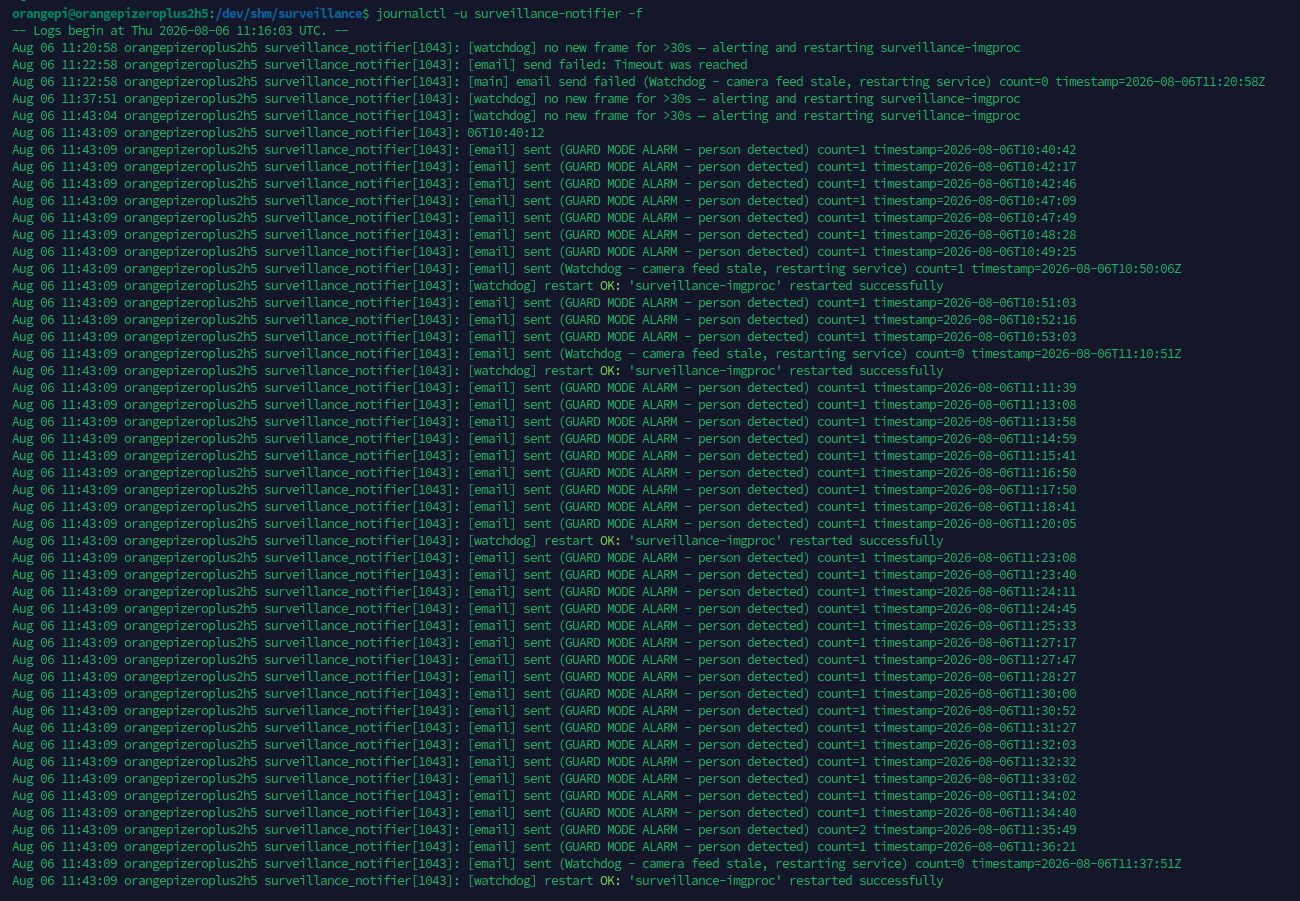
\includegraphics[width=0.95\textwidth]{../../6.Advanced Features/results/fig/GuardMode-DisconnectCamera-JournalCTL.png}
\caption{\texttt{journalctl -u surveillance-notifier -f}: the watchdog firing (\texttt{no new frame for >30s}), a genuine transient e-mail-send timeout logged \emph{without} blocking the restart, and \texttt{restart OK} confirmations for \texttt{surveillance-imgproc}.}\label{fig:watchdog-journalctl}
\end{figure}

This log is worth reading closely: at 11:20:58 the watchdog fires and
attempts to alert by e-mail, which itself times out
(\texttt{[email] send failed: Timeout was reached}) --- and the watchdog
restart proceeds anyway, logged separately as \texttt{restart OK}
moments later. \keyterm{The watchdog's core job --- recovering a stuck
detector --- does not depend on the notification succeeding.} A slow or
unreachable SMTP server is exactly the kind of transient condition a
recovery mechanism should be robust to.

\begin{table}[H]
\centering
\caption{Client-observed staleness/recovery pattern (\texttt{watchdog\_log.csv}, elapsed seconds from monitor start).}
\label{tab:watchdog-timeline}
\begin{tabular}{ll}
\toprule
\textbf{Elapsed} & \textbf{Observation} \\
\midrule
0.0\,s -- 54.4\,s & \alert{Sustained stale} --- \texttt{persons.json} timestamp not advancing \\
55.5\,s & \stable{First recovery} --- fresh frame observed \\
55.5\,s -- 178.9\,s & Intermittent recover/relapse as the HTTP-poll connection re-establishes \\
\bottomrule
\end{tabular}
\end{table}

\begin{answersection}{Reading the intermittent recovery pattern}
The first sustained stale period (0--54.4\,s) lines up with the
watchdog's 30-second timeout plus the time for
\texttt{systemctl restart} and the Python process to come back up. The
repeated brief recover/relapse cycles that follow are visible directly
in \texttt{surveillance-imgproc}'s own log
(\texttt{Connection refused}, then \texttt{HTTP Error 503: Service
Unavailable}) --- the latter is Section~\ref{sec:image-processing}'s own
laptop-side retry logic correctly reporting "camera not ready yet" rather
than failing outright, so the board keeps polling successfully into a
server that is itself still reconnecting to the webcam. The pattern is
therefore two independent retry loops (this daemon's watchdog, and
Section~\ref{sec:image-processing}'s HTTP-poll capture) settling into a
stable state together, not a fault in either one individually.
\end{answersection}

\smartsubsection{Experiment 4-4: Simulated High Temperature}
\label{sec:exp-4-4}

CPU load was driven with \texttt{stress} (\texttt{--stress-workers 4},
i.e.\ all four Cortex-A53 cores) for a 180-second window inside a
300-second sampling run, once with the board's cooling fan disconnected
and once with it attached, to obtain a clean before/after comparison of
the thermal-management response.

\begin{figure}[H]
\centering
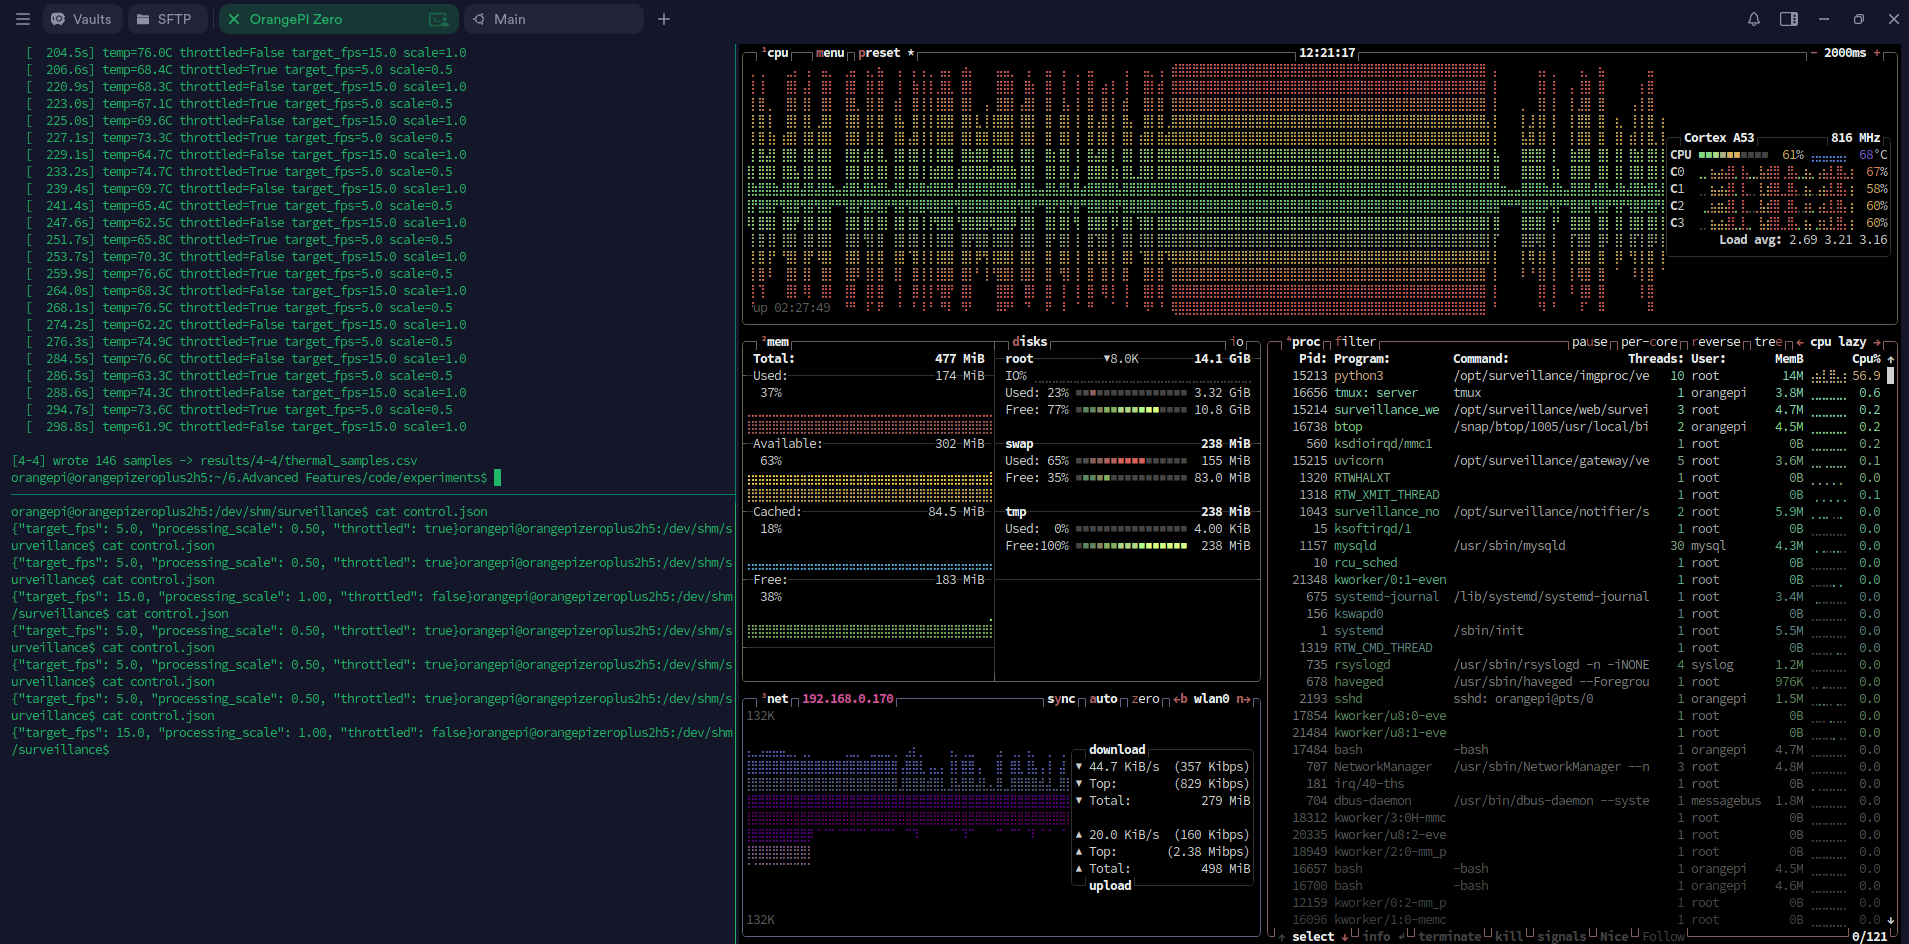
\includegraphics[width=0.95\textwidth]{../../6.Advanced Features/results/fig/NoFan-Throttled-Board.png}
\caption{No fan: local \texttt{btop} confirming genuine hardware load (CPU 61\%, 68\,°C) while \texttt{control.json} visibly toggles \texttt{throttled} between \texttt{true} and \texttt{false} in real time.}\label{fig:nofan-board}
\end{figure}

\begin{figure}[H]
\centering
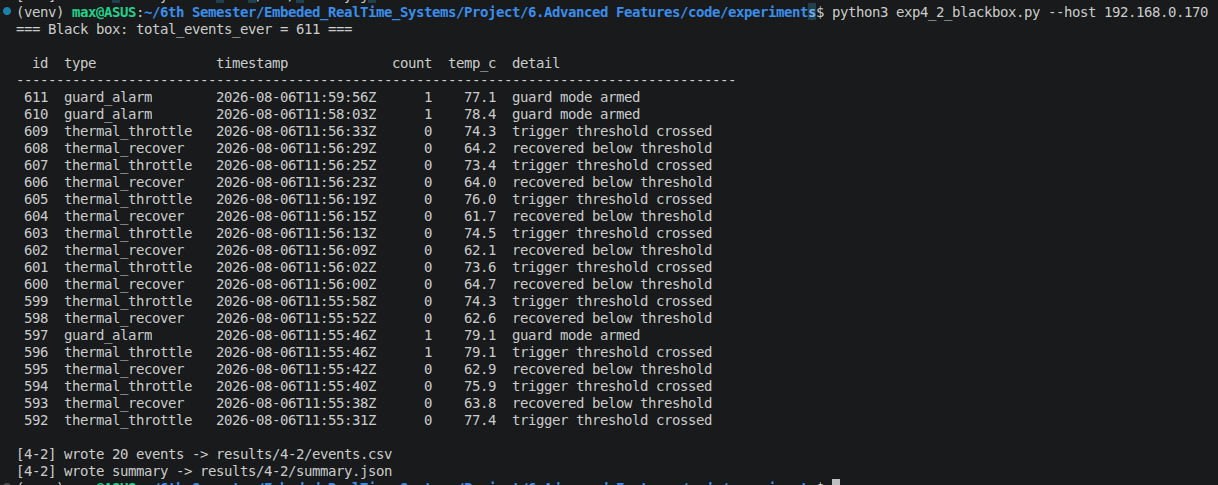
\includegraphics[width=0.95\textwidth]{../../6.Advanced Features/results/fig/NoFan-Throttled-BlackBox.png}
\caption{No fan: black-box query showing alternating \texttt{thermal\_throttle}/\texttt{thermal\_recover} events during the stress window.}\label{fig:nofan-blackbox}
\end{figure}

\begin{table}[H]
\centering
\caption{Experiment 4-4 summary: 300\,s run, \texttt{stress} active for 180\,s of it (t$\approx$20--200\,s).}
\label{tab:thermal-summary}
\begin{tabular}{lccc}
\toprule
\textbf{Configuration} & \textbf{Temp.\ range} & \textbf{Throttle events} & \textbf{Ever throttled?} \\
\midrule
No fan & \alert{61.5\,°C -- 79.7\,°C} & 15 throttle / 15 recover & \alert{Yes} \\
With fan & \stable{38.2\,°C -- 46.3\,°C} & 0 & \stable{No} \\
\bottomrule
\end{tabular}
\end{table}

\begin{figure}[H]
\centering
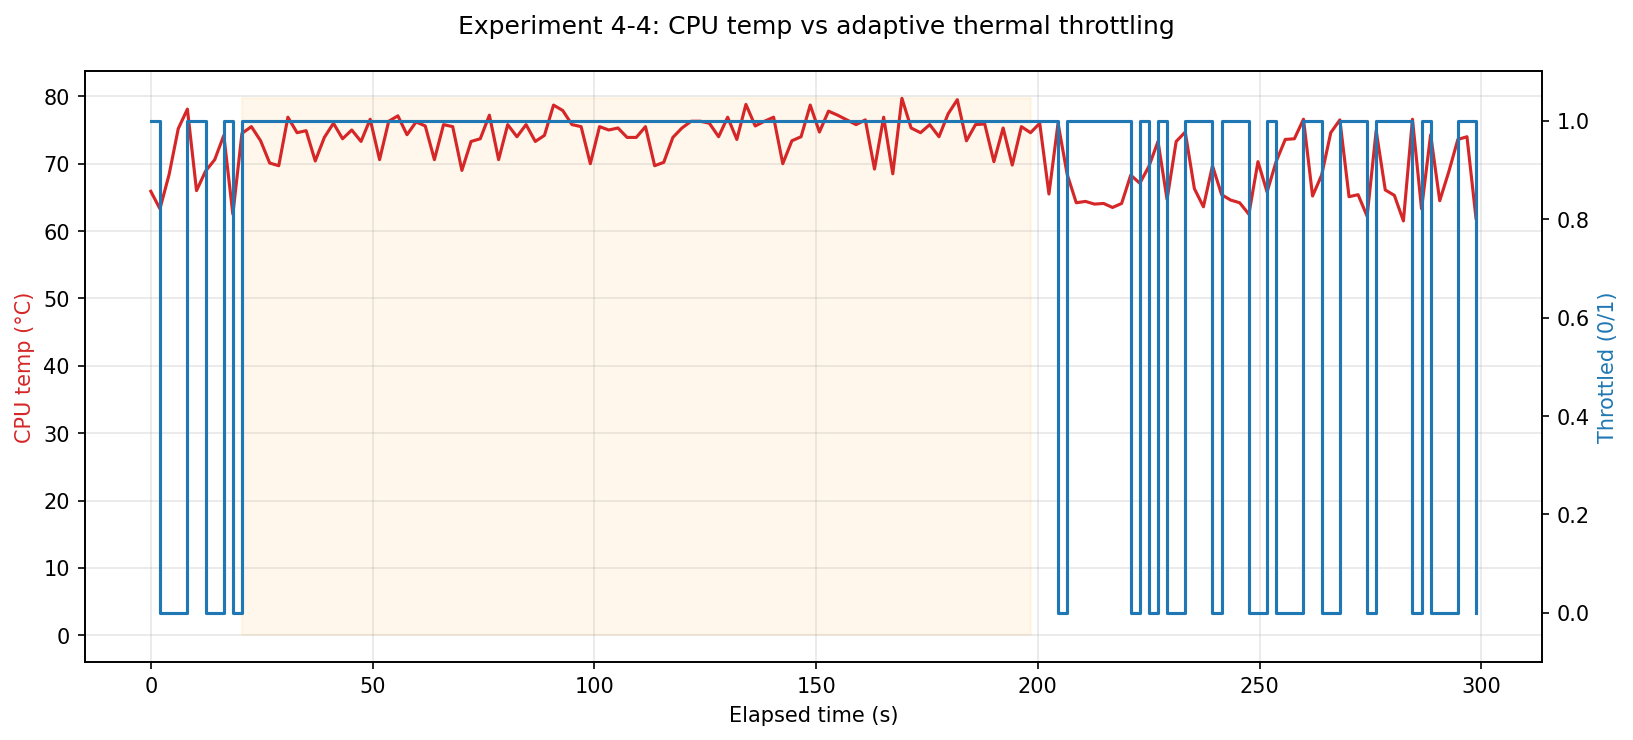
\includegraphics[width=0.9\textwidth]{../../6.Advanced Features/code/experiments/results/4-4/NoFan-exp4_4_thermal.png}
\caption{No fan: temperature (red) vs.\ throttled state (blue) over the full run. The board is continuously throttled through nearly the entire stress window (shaded), then oscillates across the hysteresis band during cooldown as temperature settles near the 65--70\,°C boundary.}\label{fig:nofan-thermal-graph}
\end{figure}

\begin{figure}[H]
\centering
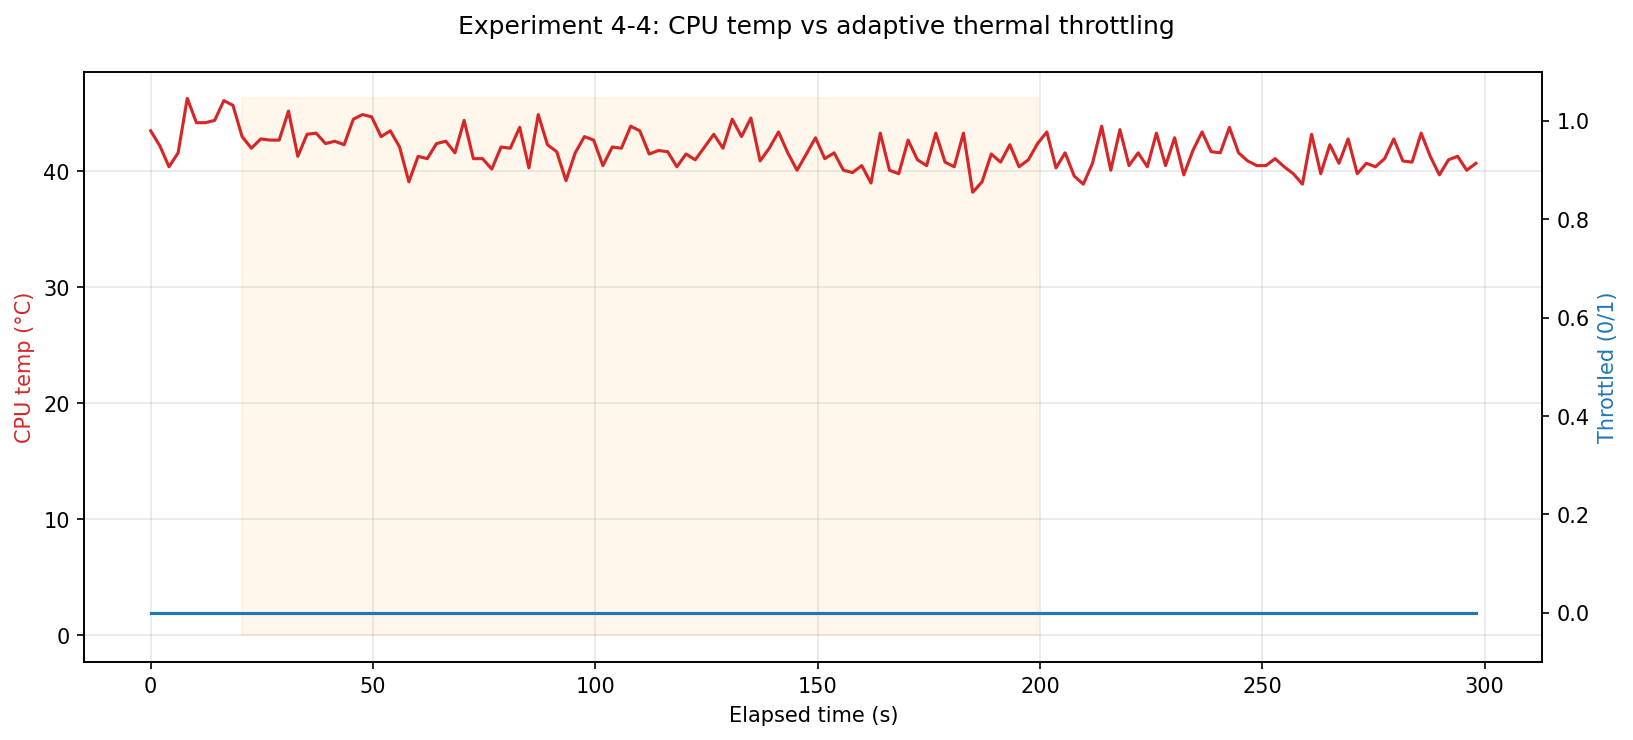
\includegraphics[width=0.9\textwidth]{../../6.Advanced Features/code/experiments/results/4-4/Fan-exp4_4_thermal.png}
\caption{With fan: temperature stays flat in the 38--46\,°C range throughout, well clear of the 70\,°C trigger --- throttling never engages.}\label{fig:fan-thermal-graph}
\end{figure}

\begin{questionsection}{Does the adaptive thermal response actually behave as designed under real, sustained load?}
The assignment asks for screenshots/logs demonstrating the adaptive
response to simulated high temperature.
\end{questionsection}

\begin{answersection}{Yes, with one honest observation about the cooldown phase}
The no-fan run demonstrates the mechanism working exactly as intended
during active load: temperature climbs past 70\,°C almost immediately
under \texttt{stress}, throttling engages and holds continuously for
essentially the entire load window, and the fan-equipped control run
under identical CPU load never approaches the trigger threshold at all
--- a clean causal demonstration that the throttling response tracks
genuine thermal load rather than some unrelated signal. The one point
worth flagging honestly: during the \emph{cooldown} phase (load removed,
temperature drifting down through the 65--70\,°C band), the system
oscillates between throttled and normal several times in quick
succession (Table~\ref{tab:thermal-summary}, Figure~\ref{fig:nofan-thermal-graph}).
This is the expected behavior of any hysteresis controller whose input
happens to hover for an extended period right at one of its two
thresholds --- the 5\,°C gap prevents chatter at a \emph{single} boundary
crossing, but does not prevent settling into a slow oscillation if the
temperature genuinely lingers across the whole band for tens of seconds
during cooldown. A wider gap (e.g.\ 70\,°C/60\,°C) would reduce this
further, at the cost of staying throttled slightly longer after a real
event before being allowed to recover --- a reasonable trade-off to
revisit if this were deployed for longer, sustained workloads rather than
demonstrated in a single test run.
\end{answersection}

\smartsubsection{Section Summary}

\begin{table}[H]
\centering
\caption{Advanced Features deliverables completed in this section.}
\label{tab:advanced-summary}
\begin{tabular}{ll}
\toprule
\textbf{Item} & \textbf{Status} \\
\midrule
Guard Mode (toggle + immediate email/MQTT alarm) & Complete \\
Black box (SQLite, circular buffer + total-ever counter) & Complete \\
Software watchdog ($>$30s stale $\to$ alert + restart) & Complete \\
Adaptive thermal management (hysteresis-based) & Complete \\
Exp.\ 4-1 (Guard Mode demo) & Complete --- Table~\ref{tab:guard-alarm-log} \\
Exp.\ 4-2 (black box contents) & Complete --- Table~\ref{tab:blackbox-events} \\
Exp.\ 4-3 (watchdog vs.\ disconnected camera) & Complete --- Figure~\ref{fig:watchdog-journalctl} \\
Exp.\ 4-4 (simulated high temperature) & Complete --- Table~\ref{tab:thermal-summary} \\
\bottomrule
\end{tabular}
\end{table}
